\documentclass[../mathNotesPreamble]{subfiles}

\providecommand{\relscalefact}{1.4}
\begin{document}
\relscale{\relscalefact}
  \section{3.4: Comparing Measures of Center}
    \begin{center}
      \begin{tabular}{@{}*{2}{c@{\hspace*{15mm}}}c@{}}\toprule
        \textbf{Shape}& \textbf{Measure for center}& \textbf{Measure for spread}\\\midrule
        Symmetric& Mean& Standard deviation\\
        Skewed& Median& IQR\\\bottomrule
      \end{tabular}
    \end{center}
    \vspace*{\stretch{1}}

    \begin{itemize}
      \item Skewed data and outliers affect the mean and standard deviation
      \item The median is resistant to outliers; it is not affected by the size of an outlier
    \end{itemize}
    \vspace*{\stretch{1}}

    \begin{center}
      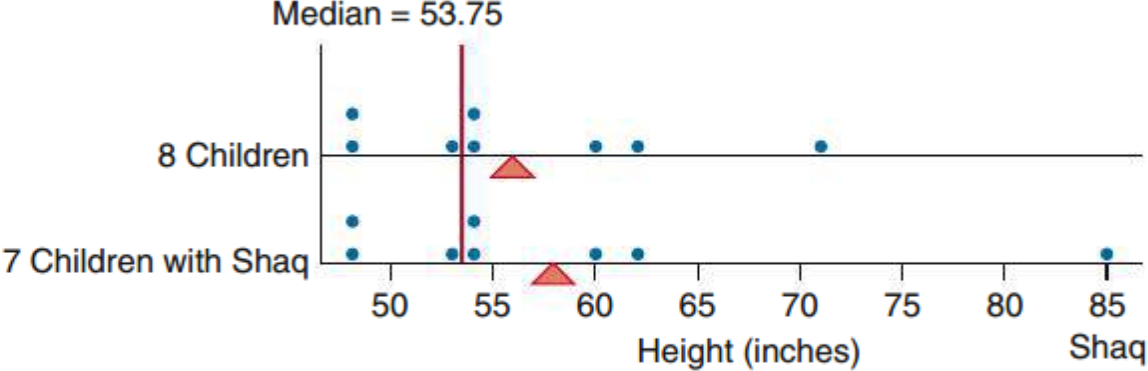
\includegraphics[width=0.75\linewidth]{images/math211_figure_3p25}
    \end{center}
    \vspace*{\stretch{1}}

    \begin{center}
      \begin{tabular}{@{}c@{\hspace*{20mm}}c@{}}\toprule
        \textbf{Shape}& \textbf{Mean vs. Median} \\\midrule
        Skewed left& Mean $<$ Median\\
        Symmetric& Mean $=$ Median\\
        Skewed right& Mean $>$ Median\\\bottomrule
      \end{tabular}
      \vspace*{\baselineskip}

      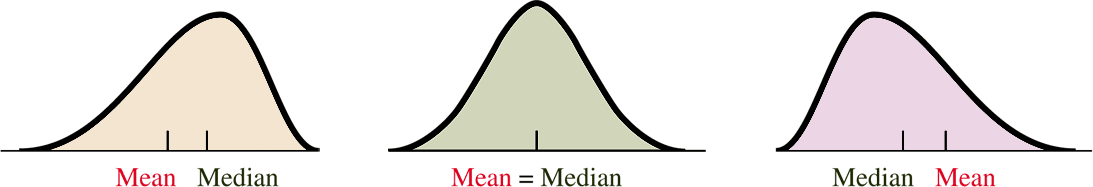
\includegraphics[width=0.85\linewidth]{images/math211_skewed_vs_symm}
    \end{center}
    \pagebreak

    \begin{ex*}
      A (very small) fast-food restaurant has five employees, all of whom work full-time for \$7 per hour. Each employee’s annual income is about \$16,000 per year. The owner, on the other hand, makes \$100,000 per year.

Find both the mean and the median. Which would you use to represent the typical income at this business -- the mean or the median?  Which value is smaller?
    \end{ex*}
    \vspace*{\baselineskip}

    \begin{center}
      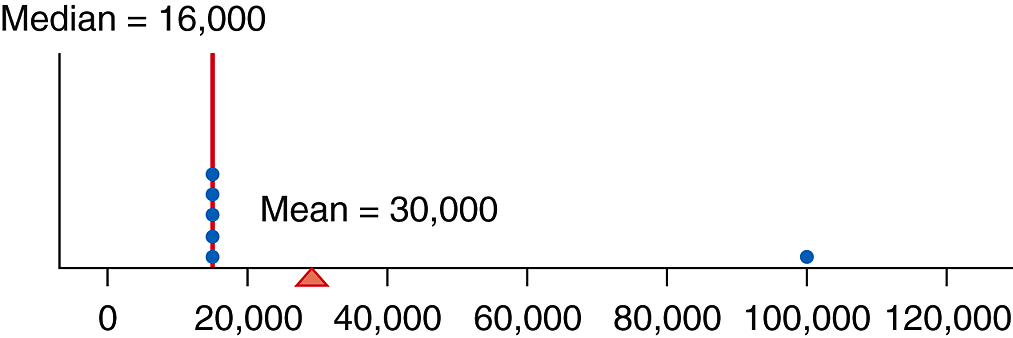
\includegraphics[width=0.75\linewidth]{images/math211_figure_3p26}
    \end{center}
    \vspace*{\stretch{1}}

    \noindent
    When comparing distributions:
    \begin{itemize}
      \item Always use the same measures of center and spread for both distributions.
      \item If one of the distributions is skewed, use Median and IQR to compare both!
    \end{itemize}
    \pagebreak

    \begin{ex*}
      Below is a histogram of the finishing times of female marathon runners.
    \end{ex*}
    \begin{center}
      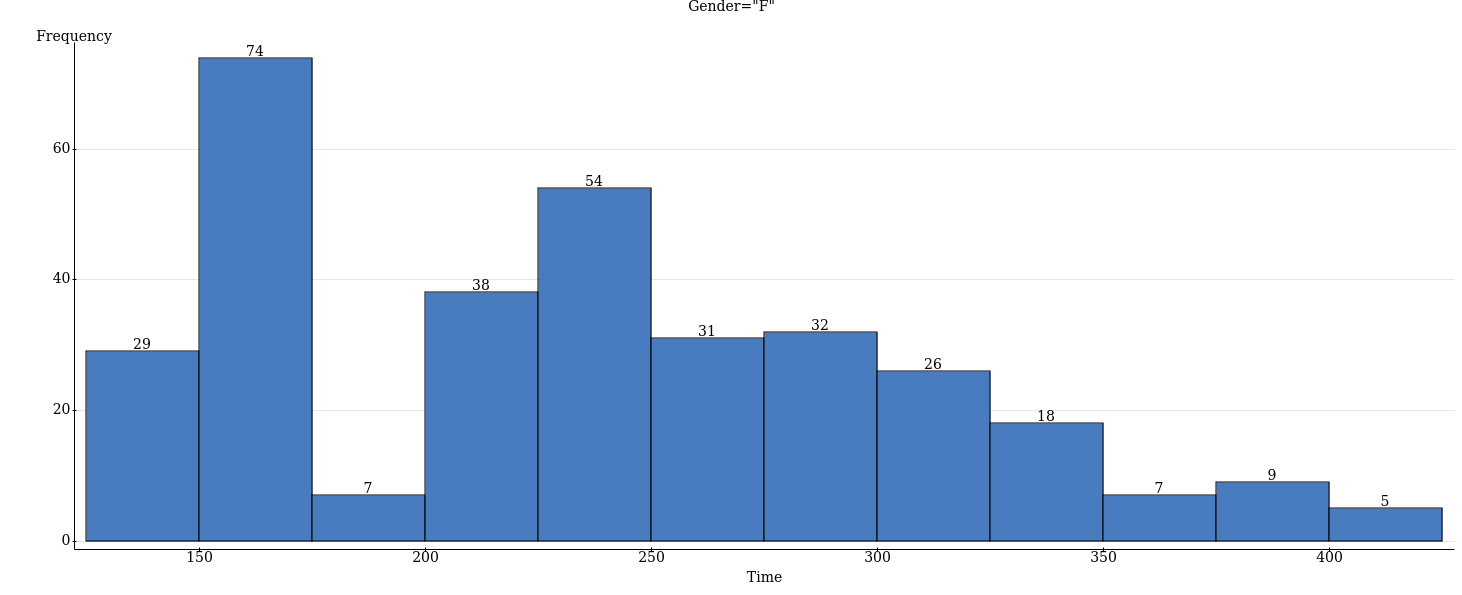
\includegraphics[width=0.65\linewidth]{images/math211_3p4_female_marathon_times}
    \end{center}
    If we separate the data into the ``Amateur'' and ``Olympic'' events, we see why the data is bimodal. If we compare the distributions, should we use the Mean or the Median? Should we use the standard deviation, or the IQR?

    \vspace*{\stretch{1}}
    \begin{center}
      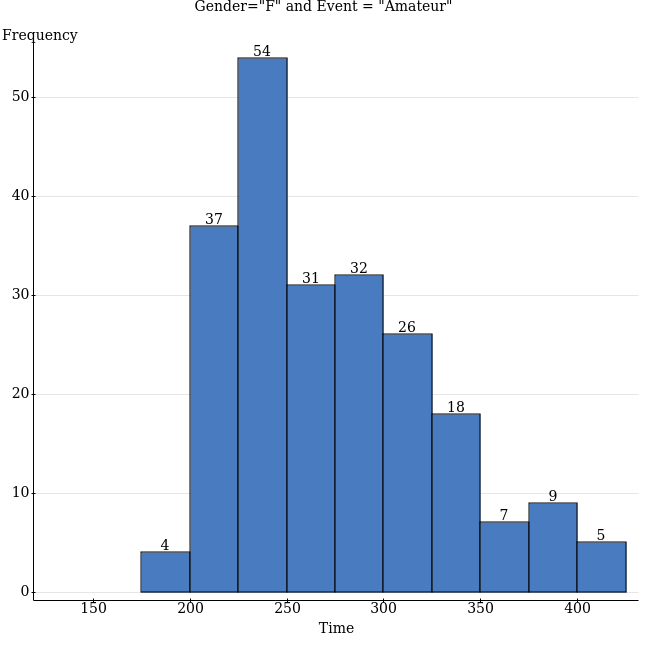
\includegraphics[width=0.45\linewidth]{images/math211_3p4_female_marathon_amateur_times}
      \hspace*{\stretch{1}}
      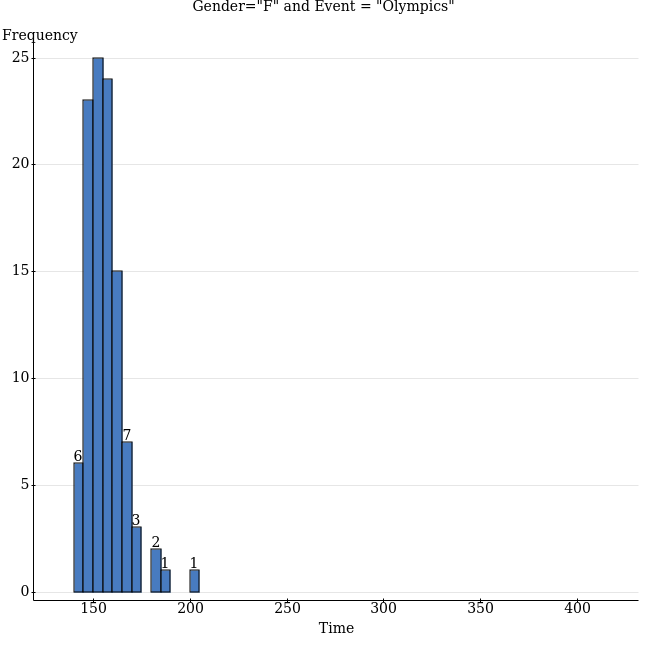
\includegraphics[width=0.45\linewidth]{images/math211_3p4_female_marathon_olympic_times}
    \end{center}

  \pagebreak
\end{document}
